\section{Exercises}

%%__________________
%\subsection{Examining the Central Limit Theorem}

% 33

\eoce{\qt{Ages of pennies, Part I} \label{penniesAges} The histogram below shows the distribution of ages of pennies at a bank. 

\noindent\begin{minipage}[c]{0.5\textwidth}
\begin{parts}
\item Describe the distribution.
\item Sampling distributions for means from simple random samples of 5, 30, and 100 pennies is shown in the histograms below. Describe the shapes of these distributions and comment on whether they look like what you would expect to see based on the Central Limit Theorem.
\end{parts}\vspace{3mm}
\end{minipage}
\begin{minipage}[c]{0.5\textwidth}
\begin{center}
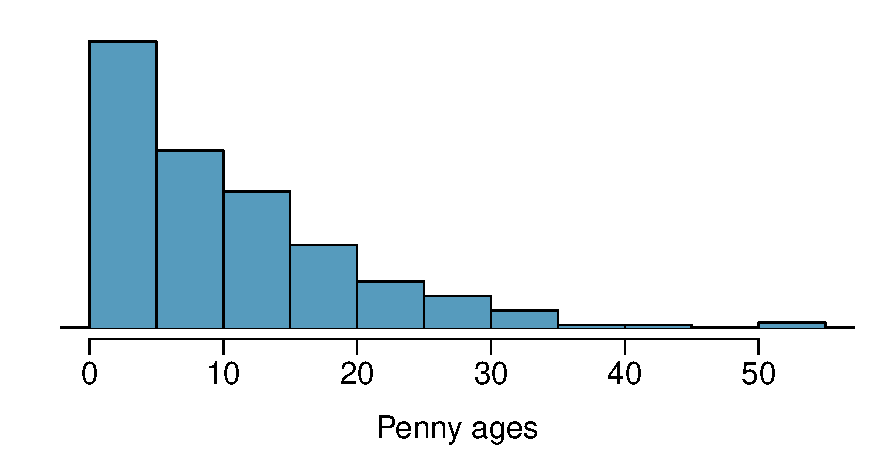
\includegraphics[width=\textwidth]{03-5/figures/eoce/penniesAges/penniesAges_pop} 
\end{center}
\end{minipage}\vspace{-1mm}
\begin{center}
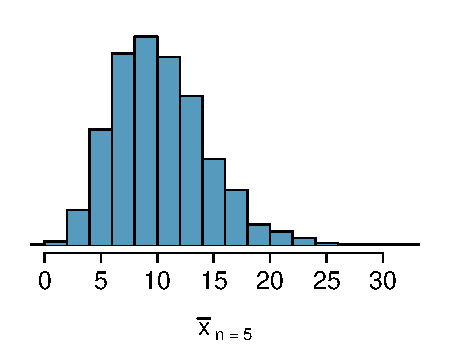
\includegraphics[width=0.325\textwidth]{03-5/figures/eoce/penniesAges/penniesAges_n5} 
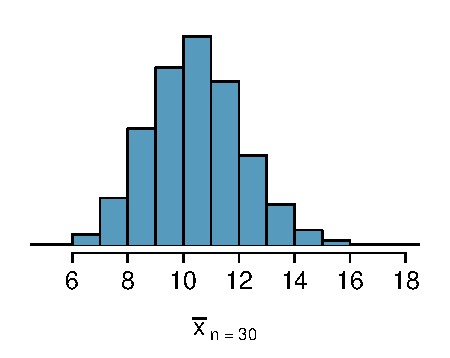
\includegraphics[width= 0.325\textwidth]{03-5/figures/eoce/penniesAges/penniesAges_n30} 
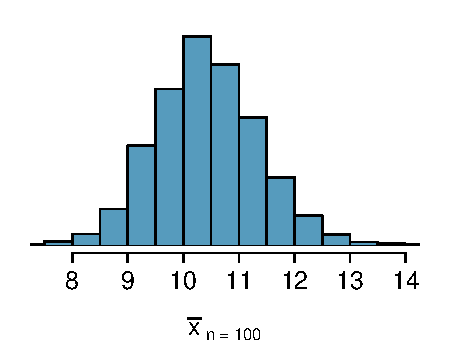
\includegraphics[width= 0.325\textwidth]{03-5/figures/eoce/penniesAges/penniesAges_n100} 
\end{center}
}{}

% 34

\eoce{\qt{Ages of pennies, Part II} The mean age of the pennies from Exercise~\ref{penniesAges} is 10.44 years with a standard deviation of 9.2 years. Using the Central Limit Theorem, calculate the means and standard deviations of the distribution of the mean from random samples of size 5, 30, and 100. Comment on whether the sampling distributions shown in Exercise~\ref{penniesAges} agree with the values you compute.
}{}

% 35

\eoce{\qt{Identify distributions, Part I} Four plots are presented below. The plot at the top is a distribution for a population. The mean is 10 and the standard deviation is 3. Also shown below is a distribution of (1) a single random sample of 100 values from this population, (2) a distribution of 100 sample means from random samples with size 5, and (3) a distribution of 100 sample means from random samples with size 25. Determine which plot (A, B, or C) is which and explain your reasoning.
\begin{center}
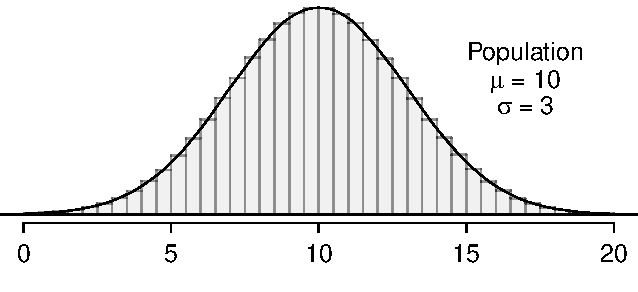
\includegraphics[width=0.5\textwidth]{03-5/figures/eoce/cltSimSYM/cltSimSYM_pop}
\end{center}
\begin{center}
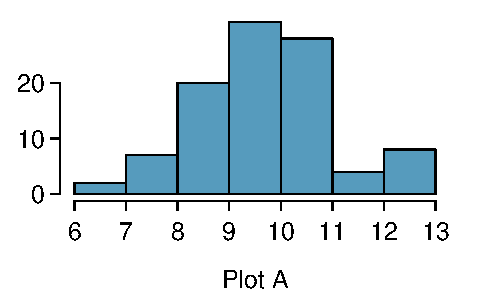
\includegraphics[width=0.32\textwidth]{03-5/figures/eoce/cltSimSYM/cltSimSYM_n5}
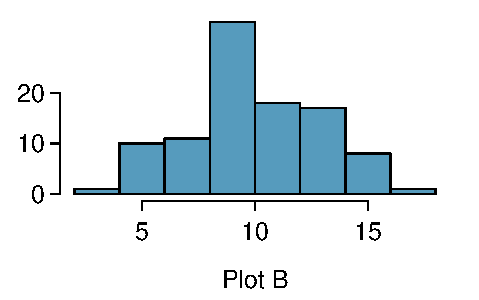
\includegraphics[width=0.32\textwidth]{03-5/figures/eoce/cltSimSYM/cltSimSYM_samp}
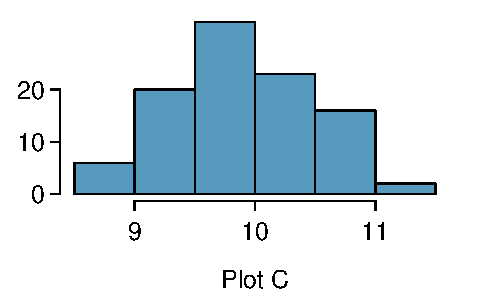
\includegraphics[width=0.32\textwidth]{03-5/figures/eoce/cltSimSYM/cltSimSYM_n25}
\end{center}
}{}

% 36

\eoce{\qt{Identify distributions, Part II} Four plots are presented below. The plot at the top is a distribution for a population. The mean is 60 and the standard deviation is 18. Also shown below is a distribution of (1) a single random sample of 500 values from this population, (2) a distribution of 500 sample means from random samples of each size 18, and (3) a distribution of 500 sample means from random samples of each size 81. Determine which plot (A, B, or C) is which and explain your reasoning.
\begin{center}
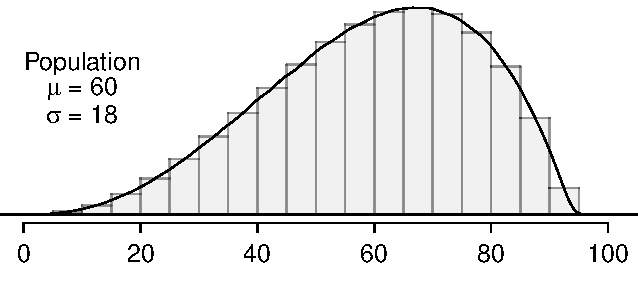
\includegraphics[width=0.5\textwidth]{03-5/figures/eoce/cltSimLS/cltSimLS_pop}
\end{center}
\begin{center}
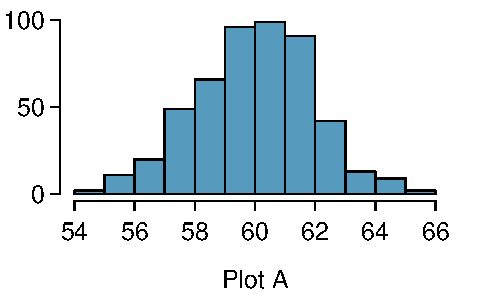
\includegraphics[width=0.32\textwidth]{03-5/figures/eoce/cltSimLS/cltSimLS_n81}
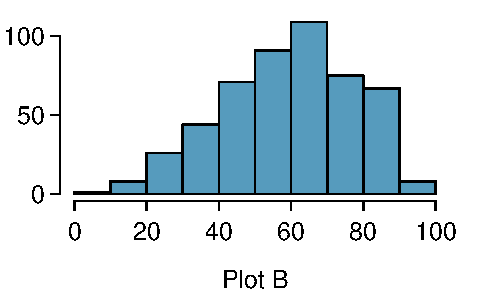
\includegraphics[width=0.32\textwidth]{03-5/figures/eoce/cltSimLS/cltSimLS_samp}
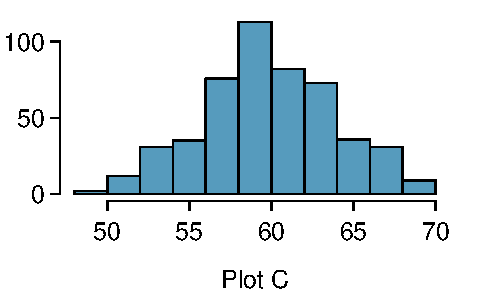
\includegraphics[width=0.32\textwidth]{03-5/figures/eoce/cltSimLS/cltSimLS_n18}
\end{center}
}{} 

% 37

\eoce{\qt{Housing prices, Part I} \label{Topanga} A housing survey was conducted to determine the price of a typical home in Topanga, CA. The mean price of a house was roughly \$1.3 million with a standard deviation of \$300,000. There were no houses listed below \$600,000 but a few houses above \$3 million.
\begin{parts}
\item Is the distribution of housing prices in Topanga symmetric, right skewed, or left skewed? \textit{Hint:} Sketch the distribution.
\item Would you expect most houses in Topanga to cost more or less than \$1.3 million?
\item Can we estimate the probability that a randomly chosen house in Topanga costs more than \$1.4 million using the normal distribution?
\item What is the probability that the mean of 60 randomly chosen houses in Topanga is more than \$1.4 million?
\item How would doubling the sample size affect the standard error of the mean?
\end{parts}
}{}

% 38

\eoce{\qt{Stats final scores} Each year about 1500 students take the introductory statistics course at a large university. This year scores on the final exam are distributed with a median of 74 points, a mean of 70 points, and a standard deviation of 10 points. There are no students who scored above 100 (the maximum score attainable on the final) but a few students scored below 20 points.
\begin{parts}
\item Is the distribution of scores on this final exam symmetric, right skewed, or left skewed?
\item Would you expect most students to have scored above or below 70 points?
\item Can we calculate the probability that a randomly chosen student scored above 75 using the normal distribution?
\item What is the probability that the average score for a random sample of 40 students is above 75?
\item How would cutting the sample size in half affect the standard error of the mean?
\end{parts}
}{}

% 39

\eoce{\qt{Weights of pennies} The distribution of weights of US pennies is approximately normal with a mean of 2.5 grams and a standard deviation of 0.03 grams.
\begin{parts}
\item What is the probability that a randomly chosen penny weighs less than 2.4 grams?
\item Describe the sampling distribution of the mean weight of 10 randomly chosen pennies.
\item What is the probability that the mean weight of 10 pennies is less than 2.4 grams?
\item Sketch the two distributions (population and sampling) on the same scale.
\item Could you estimate the probabilities from (a) and (c) if the weights of pennies had a skewed distribution?
\end{parts}
}{}

% 40

\eoce{\qt{CFLs} A manufacturer of compact fluorescent light bulbs advertises that the distribution of the lifespans of these light bulbs is nearly normal with a mean of 9,000 hours and a standard deviation of 1,000 hours.
\begin{parts}
\item What is the probability that a randomly chosen light bulb lasts more than 10,500 hours?
\item Describe the distribution of the mean lifespan of 15 light bulbs. 
\item What is the probability that the mean lifespan of 15 randomly chosen light bulbs is more than 10,500 hours?
\item Sketch the two distributions (population and sampling) on the same scale.
\item Could you estimate the probabilities from parts~(a) and~(c) if the lifespans of light bulbs had a skewed distribution?
\end{parts}
}{}

%\textB{\newpage}

% 41

\eoce{\qt{Songs on an  iPod} Suppose an iPod has 3,000 songs. The histogram below shows the distribution of the lengths of these songs. We also know that, for this iPod, the mean length is 3.45 minutes and the standard deviation is 1.63 minutes. 
\begin{center}
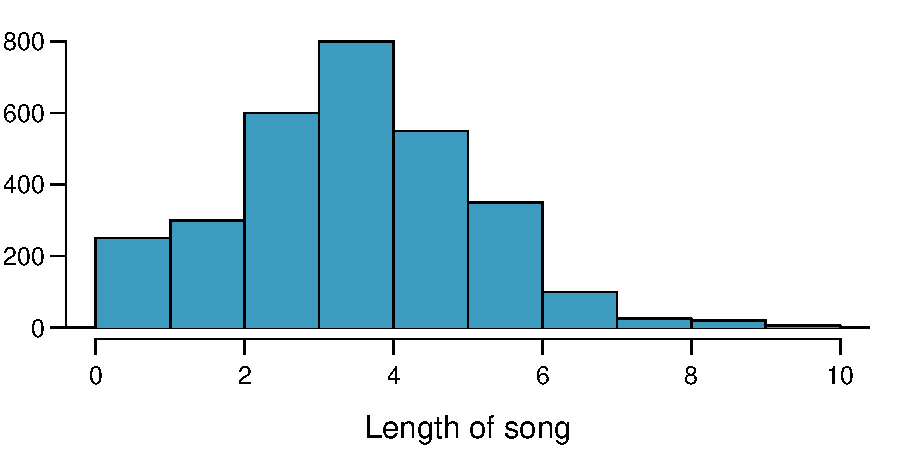
\includegraphics[width=0.75\textwidth]{03-5/figures/eoce/ipod/ipod_popdist}
\end{center}
\begin{parts}
\item Calculate the probability that a randomly selected song lasts more than 5 minutes.
\item You are about to go for an hour run and you make a random playlist of 15 songs. What is the probability that your playlist lasts for the entire duration of your run? \textit{Hint:} If you want the playlist to last 60 minutes, what should be the minimum average length of a song?
\item You are about to take a trip to visit your parents and the drive is 6 hours. You make a random playlist of 100 songs. What is the probability that your playlist lasts the entire drive?
\end{parts}
}{}

% 42

\eoce{\qt{Spray paint} Suppose the area that can be painted using a single can of spray paint is slightly variable and follows a nearly normal distribution with a mean of 25 square feet and a standard deviation of 3 square feet. 
\begin{parts}
\item What is the probability that the area covered by a can of spray paint is more than 27 square feet?
\item Suppose you want to spray paint an area of 540 square feet using 20 cans of spray paint. On average, how many square feet must each can be able to cover to spray paint all 540 square feet?
\item What is the probability that you can cover a 540 square feet area using 20 cans of spray paint?
\item If the area covered by a can of spray paint had a slightly skewed distribution, could you still calculate the probabilities in parts~(a) and~(c) using the normal distribution?
\end{parts}
}{}


\textB{\newpage}